\chapter{External Interface Requirements}

\section{User Interfaces}

The \acrshort{csaf}  package exists as middleware. It exists as a library, and no CLI or GUI tools are planned.

\section{Software Interfaces}

\subsection{Mathematical Representation}
A component is required to be a dynamical system in some form, a mathematical entity that has the ability to 
evolve in time. This means that a system assumes a function in a set $\left\{ f^t \right\}_{t \in \mathbb F}$, 
where $\mathbb F$ is some field for time. For continuous time systems, this field can be the real numbers $
\mathbb R$; for discrete, the integers $\mathbb Z$ suffices. For systems that use both discrete and 
continuous time, a relation between the two fields is necessary. A sampling frequency and sampling phase is 
used if the discrete time system is uniform time step. This general form, a system as a set of functions, is not 
conducive towards using in a software system, and another representation is desired. \\

Commonly, the set of functions can be shown as a solutions to a system of ordinary differential equations 
(\acrshort{ode}s) for continuous time or ordinary difference equations for discrete time. These systems of 
equations can be put into a form that permit a common programmatic representation. For continuous time,

\begin{equation}
\begin{cases}
\dot x = g(t, x, u; p) \\
f_{x_0}^t = h(., x(.), u; r) \\
\end{cases}
\end{equation}

This form separates the solution into two steps with respect to an initial condition $x_0$. First, all variables 
where the \acrshort{ode}s involve rates of change are grouped in a vector $x \in \mathbb R^N$, where it 
assumes an element in a state space. $u \in \mathbb R^M$ is an additional time varying vector, representing 
control input to the system. $p$ and $r$ are time independent parameters involved with the two functions. 
Then, another function $h$ takes the space and returns the system configuration, evaluating one of the 
system functions. Similarly, a construction can be made for a discrete system,

\begin{equation}
\begin{cases}
x_{n} = g(t, n-1, u; p)\\
f^{n}_{x_0} = h(., x(.), u; r) \\
\end{cases},
\end{equation}

for the discrete time system. The evolution of the state $x$ can be computed directly rather than integrating 
the system of equations defining the state differential. Further, time itself need not be directly expressed, an 
essential parameter for non-autonomous systems. The equivalence holds

\begin{equation}
\begin{bmatrix}
\dot x \\
t
\end{bmatrix} = 
\begin{bmatrix}
g(t, x, u; p) \\
1
\end{bmatrix} \iff \dot x = g(t, x, u;p) .
\end{equation}

However, for the sake of implementation, it is advantageous to express the time parameter directly. To use 
this form, all \acrshort{csaf}  components require two functions, 

\begin{equation}
\begin{aligned}
g(.,.,.;p):& \mathbb F \times \mathbb R^N \times \mathbb R^M \rightarrow \mathbb R^N \\
h(.,.,.;r):& \mathbb F \times \mathbb R^N \times \mathbb R^M \rightarrow \mathbb R^D
\end{aligned}.
\end{equation}

For continuous time solution of a single component, the function $g(.,.,u(.);p)$ is of a form that common 
\acrshort{ode} solvers can evaluate. The parameters $r$ and $p$ don't necessarily need to be elements of a 
vector space, and can be described using other structures.

\subsection{Component Interfaces}

From the mathematical representations, a component can be described by three elements: its parameters, 
state evolution function and output function. Figure \ref{fig:cio} shows a component's IO contents, as well as 
a form that all systems must take. The incoming and outgoing data are in the form of a serial message, but 
contain the time and state information. The outgoing message contains the system output and parameters as 
well.

\begin{figure}
\centering
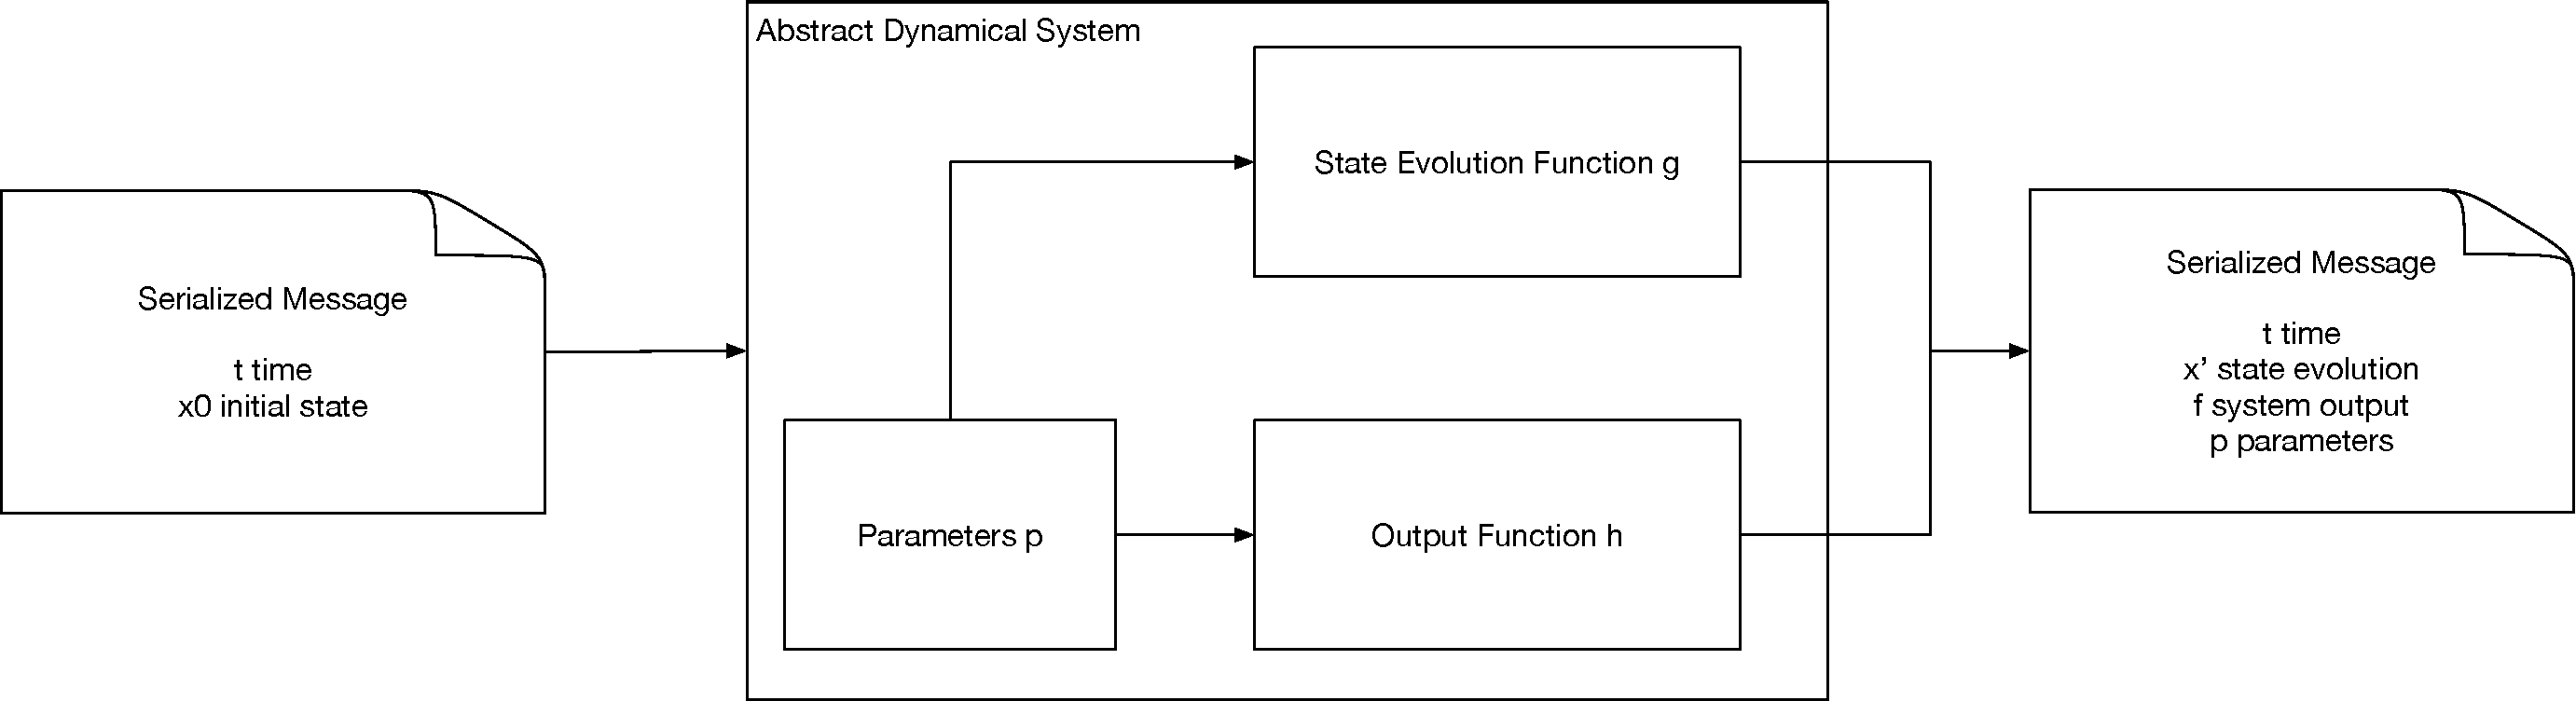
\includegraphics[width=1.0\textwidth]{componentio.pdf}
\caption{Contents of \acrshort{csaf}  Component IO}
\label{fig:cio}
\end{figure}

\section{Communications Interfaces}

Analyzers and simulators will interact with the system components via zeroMQ, using sockets. zeroMQ 
provides \acrshort{csaf}  with a variety of levels to communicate with components, whether in-process, 
inter-process or across TCP and multi-cast. The component does hold state, and the system needs to be 
properly initialized to avoid staleness.

\subsection{Message Contents}

The temporal messages sent by every \acrshort{csaf}  component needs to have specific content to support 
simulation. The message type is derived from the \acrshort{ros} message serialization format. First, the the 
\acrshort{csaf}  version is transmitted to avoid incompatibility between components made with different 
versions. Second, an epoch is included to keep a record on how many publish events have been performed 
by a component. Temporal information is included, being time and sampling frequency. Next is the input, 
output and state vectors. These vectors are enumerated under a header, rather than transmitted as a 
contiguous array. Figure \ref{fig:cmsg} shows an example message. \\

A component has another sub/pub pair that allows non-temporal aspects of the system to be configured. 
Invariant parameters of the system can be named and be received and set. The system name, representation 
identifier and solver name is included as a string. Two booleans are used to determine if the 
system type---continuous, discrete or hybrid.  Fields specific to the representation of the system is 
accessible. For example, if the system is a fuzzy controller, the inference table can be visible. As the 
components have a varying degree of transparency (``black box''), no headers are required and parameters 
are allowed to unchangeable. \\

What is required from a component is dependent on its representation and its purpose. As such, much 
variability can exist in what is contained in the message. New headers and variables are allowed to appear in a 
component message, but the structure has to remain constant over time. \\

\begin{figure}
\begin{lstlisting}
uint32 version_major
uint32 version_minor

uint32 epoch

Header Input
	float64 input1
	float64 input2
	
Header Output
	float64 output1
	float64 output2
	
Header State
	float64 state1
	float64 state2
	
Header Differential
	float64 stated1
	float64 stated2
\end{lstlisting}
\caption{Required \acrshort{csaf}  Component Temporal Message Contents (Other Fields are Permitted)}
\label{fig:cmsg}
\end{figure}

\begin{figure}
\begin{lstlisting}
uint32 version_major
uint32 version_minor

uint32 epoch

string system_name
string system_representation
string system_solver

float64 time
float64 sampling_frequency

bool is_discrete
bool is_hybrid


Header Parameters
	float64 input1
	float64 input2
	
Header ParameterNames
	string pname1
	string pname2
	
Header InitialState
	float64 istate1
	float64 istate2
	
Header StateNames
	string sname1
	string sname2
\end{lstlisting}
\caption{Required \acrshort{csaf}  Component Information Message Contents (Other Fields are Permitted)}
\label{fig:cmsg}
\end{figure}

